\documentclass[a4paper,12pt]{article}

% рисунки
\usepackage{graphicx}

\usepackage[T2A]{fontenc}
\usepackage[utf8]{inputenc}
\usepackage[english,russian]{babel}

\RequirePackage{caption}
\DeclareCaptionLabelSeparator{defffis}{ — }
\captionsetup{justification=centering,labelsep=defffis}

\usepackage{caption} \captionsetup[table]{labelsep=endash,justification=justified,singlelinecheck=false,font=normalsize}

\usepackage{amsmath,amsfonts,amssymb,amsthm,mathtools}



\begin{document}
  
\begin{center}
  \section*{Лабораторная работа №3.4.1 \\Диа- и парамагнетики \\Джокер Бэтмен, Б02-000, 12.09.2021}
\end{center}  

\vspace{5mm}
\section*{Введение}

\begin{flushleft}
  \textbf{Цель работы:} измерение магнитной восприимчивости диа- и парамагнитных образцов.
\end{flushleft}

\begin{flushleft}
  \textbf{В работе используются:} электромагнит, аналитические весы, милливеберметр, регулируемый источник постоянного тока, образцы.
\end{flushleft}

\section*{Теоретическая справка}

Магнитная восприимчивость тел может быть определена по измерению сил, действующих на тела в магнитном поле. Одним из классических методов таких измерений является т.н. \textit{метод Гюи}. В нём используется длинный тонкий стержень, один из концов которого помещают в зазор электромагнита (обычно в область однородного поля), а другой конец -- вне зазора, где величиной магнитного поля можно пренебречь. В этом случае закон изменения поля -- от максимального до нулевого -- будет несущественен.

Найдём выражение для силы, действующей со стороны магнитного поля на помещённый в зазор электромагнита цилиндрический стержень. Пусть площадь его сечения равна $S$, его магнитная проницаемость -- $\mu$, поле в зазоре -- $B_0$, а глубина, на которую стержень помещён в зазор, -- $x$. Так как ток $I$ через электромагнит остаётся постоянным, то сила, действующая на стержень со стороны магнитного поля, равна производной магнитной энергии системы по координате, взятой с противоположным знаком:\[F_M=\left(\frac{\partial W_M}{\partial x}\right)_I,\]где $W_M(x)$ -- магнитная энергия системы при $I=\text{const}$ (то есть при $B_0=\text{const}$) в зависимости от глубины погружения стержня $x$.

Объёмную плотность магнитной энергии можно найти по формуле:\[W_M=\frac{1}{2\mu_0}\int\frac{B^2}{\mu}\text{d}V,\]где интеграл берётся по всему пространству.

Найдём теперь распределение магнитного поля в цилиндре. Рассмотрим сначала бесконечный стержень с проницаемостью $\mu$, помещённый в перпендикулярное ему однородное поле $B_0=\mu_0H_0$, и найдём поле $B_{\text{ст}}$ внутри него. В силу малости магнитной восприимчивости исследуемых образцов можно воспользоваться непрерывностью касательной компоненты $H$ и считать, что внутри стержня $H_{\text{ст}}=H_0$, потому $B_{\text{ст}}=\mu B_0$. Тогда систему из стержня в зазоре электромагнита можно условно разбить на три части -- вне электромагнита (I), в погружённой части стержня (II) и в электромагните вдали от стержня (III). В области I поле мало ($B_1\approx0$), поэтому его вкладом в энергию можно пренебречь. В области II поле приближённо равно $B_2\approx\mu B_0$, а в области III -- $B_3\approx B_0$.

При смещении цилиндра вглубь электромагнита на $\text{d}x$ область II увеличивается в объёме на $\text{d}V_2=S\text{d}x$, а область III уменьшается на $\text{d}V_3=-S\text{d}x$. Распределение поля в пограничных участках между областями при этом почти не меняется. Тогда изменение магнитной энергии при таком смещении равно:\[\text{d}W_M(\text{d}x)\approx\frac{B_2^2}{2\mu\mu_0}S\text{d}x-\frac{B_2^2}{2\mu_0}S\text{d}x=\left(\mu-1\right)\frac{B_0^2}{2\mu_0}S\text{d}x.\]Следовательно, искомая сила равна:\[F_M=\left(\frac{\partial W_M}{\partial x}\right)_{B_0}\approx\chi\frac{B_0^2}{2\mu_0}S.\]

Знак силы зависит от знака восприимчивости $\chi=\mu-1$: парамагнетики ($\chi > 0$) \textit{втягиваются} в зазор электромагнита, а диамагнетики ($\chi < 0$) \textit{выталкиваются} из него. Таким образом, измерив силу, действующую на образец в магнитном поле $B_0$, можно рассчитать его магнитную восприимчивость.

\section*{Экспериментальная установка}

Схема установки показана на рисунке \Ref{Установка}. Магнитное поле с максимальной индукцией $\approx1~\text{Тл}$ создаётся в зазоре электромагнита, питаемого постоянным током. Диаметр его полюсов существенно превосходит ширину зазора, поэтому поле в его средней части достаточно однородно. Величина тока, проходящего через обмотки электромагнита, задаётся регулируемым источником постоянного тока.

\begin{figure}[h]
	\centering
	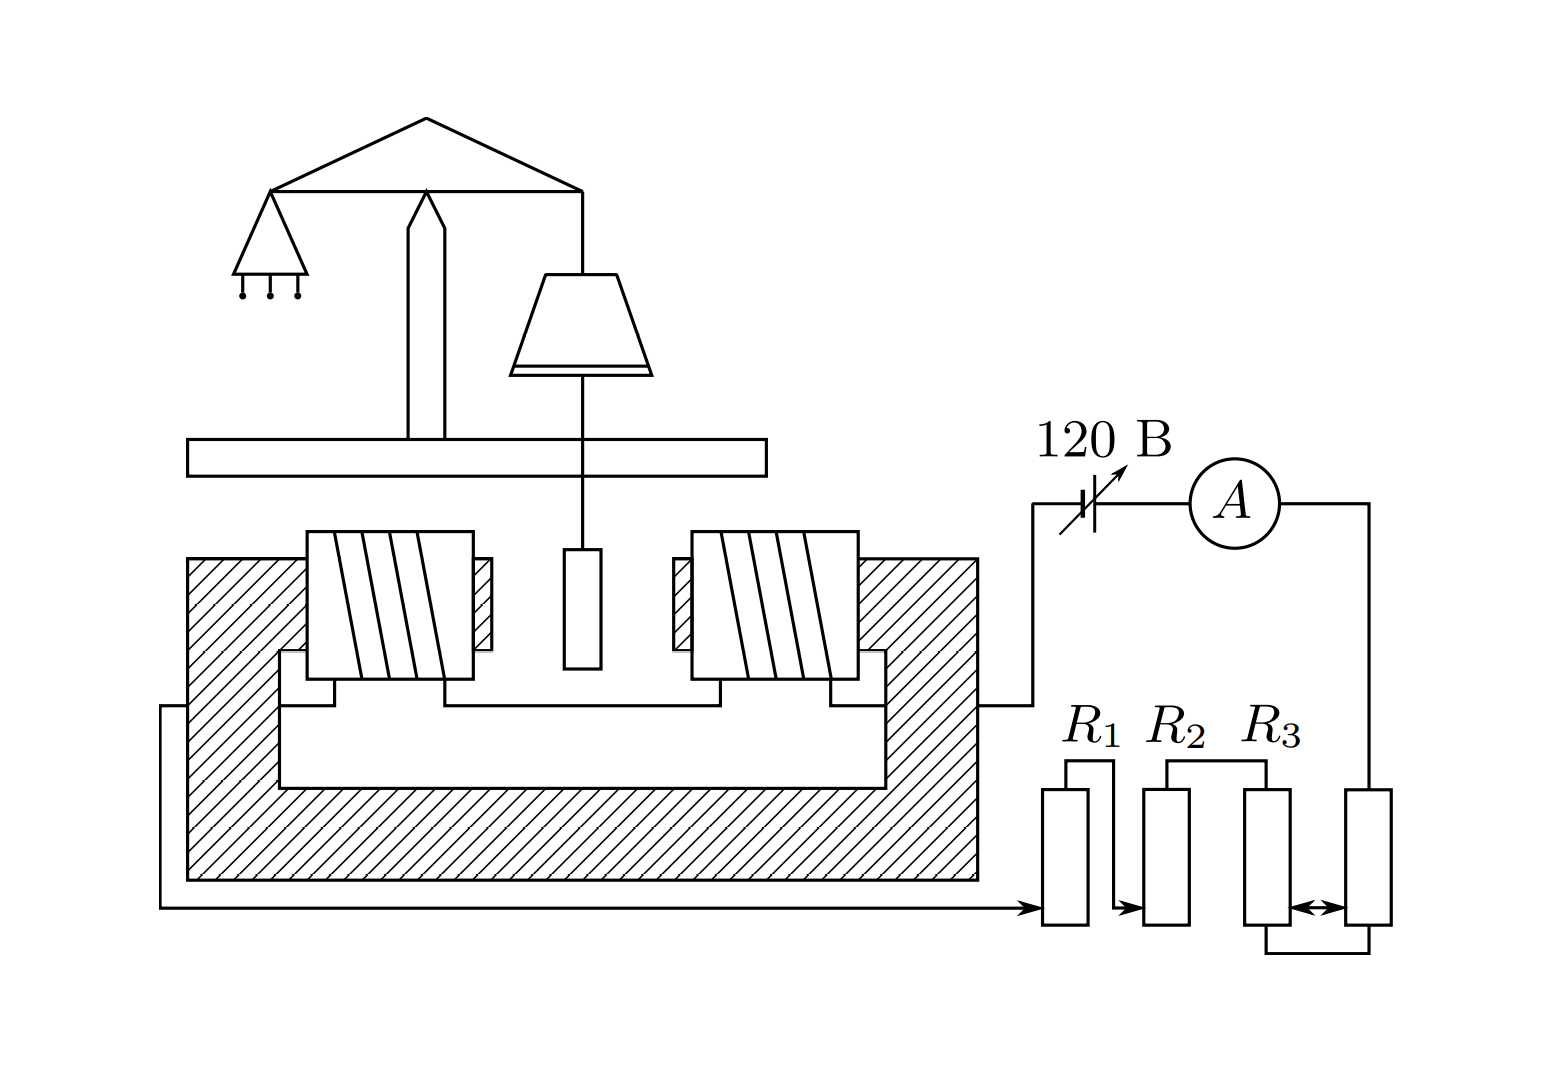
\includegraphics[scale=0.35]{Device}
	\caption{Схема экспериментальной установки} \label{Установка}
\end{figure}

Градуировка электромагнита (связь между индукцией магнитного поля $B$ в зазоре и силой тока $I$ в обмотках) производится при помощи милливеберметра. При измерениях образцы поочерёдно подвешиваются к аналитическим весам так, что один конец образца оказывается в зазоре электромагнита, а другой -- вне его, где индукцией магнитного поля можно пренебречь. При помощи аналитических весов определяется перегрузка $\Delta P=F$ -- сила, действущая на образец со стороны магнитного поля.

Погрешности приборов: милливеберметра -- половина цены деления шкалы, т.е. $\Delta\Phi=0.05~\text{мВб}$, электрических приборов -- амперметра и весов -- $0,5\%+2~\text{ед. мл. разряда}$.

\section*{Ход работы}

Убедимся, что цепь питания электромагнита работает исправно. Ток $I$, протекающий через него, меняется в диапазоне от нуля до $I_{max}=3,08~\text{А}$ (минимальное используемое в работе значение силы тока $I_{min}=0,30~\text{А}$).

Приступим к калибровке электромагнита. С помощью милливеберметра снимем зависимость магниного потока $\Phi$, пронизывающего пробную катушку, находящуюся в зазоре, от тока $I$ ($\Phi=BSN$, где значение $SN=72~\text{см}^2=7,2\cdot10^{-3}~\text{м}^2$ -- произведение площади сечения пробной катушки на число витков в ней -- указано на установке (погрешностью его пренебрежём)). Для измерения магнитного потока необходимо сначала поместить пробную катушку в зазор электромагнита и записать показания милливеберметра $\Phi_1$ при этом. Затем её нужно очень быстро убрать из зазора и записать показания милливеберметра $\Phi_2$. Разность $\Phi_1-\Phi_2$ и будет определять величину магнитного потока $\Phi$ через пробную катушку, откуда с лёгкостью можно найти соответствующую величину магнитного поля $B$. Проведём измерения при 8 различных значениях тока $I$. Все полученные данные занесём в таблицу \Ref{Калибровка}. В дальнейшем будем учитывать также погрешность милливеберметра. При измерении $\Phi=\Phi_1-\Phi_2$ погрешность равна $\sigma_{\Phi}=\sqrt{\sigma_{\Phi_1}^2+\sigma_{\Phi_2}^2}=\sqrt2\Delta\Phi$, откуда погрешность определения индукции магнитного поля равна $\sigma_B=\frac{\sigma_{\Phi}}{SN}=\frac{\sqrt2\Delta\Phi}{SN}\approx0,01~\text{Тл}$. Погрешность измерения тока будет равна $\sigma_I=0,005I+0,02~\text{А}$, также внесём её в таблицу.

\begin{table}[h]
	\centering
	\caption{Зависимость индукции магнитного поля $B$ в зазоре электромагнита от тока $I$ через обмотки} \label{Калибровка}
	\begin{tabular}{|c|c|c|c|c|c|c|c|c|}
		\hline
		$I$, А & 0,30 & 0,70 & 1,10 & 1,50 & 1,90 & 2,30 & 2,70 & 3,08 \\ \hline
		$\sigma_I$, А & 0,02 & 0,02 & 0,03 & 0,03 & 0,03 & 0,03 & 0,03 & 0,04 \\ \hline
		$\Phi_1$, мВб & 5,5 & 6,2 & 7,0 & 7,8 & 8,4 & 9,1 & 9,6 & 8,3 \\ \hline
		$\Phi_2$, мВб & 4,8 & 4,5 & 4,3 & 4,2 & 3,9 & 3,7 & 3,5 & 1,6 \\ \hline
		$\Phi$, мВб & 0,7 & 1,7 & 2,7 & 3,6 & 4,5 & 5,4 & 6,1 & 6,7 \\ \hline
		$B$, Тл & 0,10 & 0,24 & 0,38 & 0,50 & 0,63 & 0,75 & 0,85 & 0,93 \\ \hline
	\end{tabular}
\end{table}

В работе используются три образца, выполненных из меди (Cu), алюминия (Al) и графита (C). При рассчёте магнитной восприимчивости материалов $\chi$ потребуется диаметр образцов, который указан ниже в таблице \Ref{Параметры} (погрешностями этих значений пренебрежём).

\begin{table}[h]
	\centering
	\caption{Диаметр $d$ образцов, используемых в эксперименте} \label{Параметры}
	\begin{tabular}{|c|c|c|c|}
		\hline
		  & Cu & Al & C \\ \hline
		$d$, см & 1,00 & 1,00 & 0,67 \\ \hline
	\end{tabular}
\end{table}

Приступим теперь к измерению сил, действующих на образцы в магнитном поле. Не включая электромагнит, подвесим к весам один из образцов и обнулим показания весов, нажав на кнопку "TARE". Установим минимальное значение тока через электромагнит и проведём измерение равновесного значения массы $\Delta m$. Повторим эти измерения для ещё 7 значений тока, совпадающих с использованными при калибровке электромагнита, сначала увеличивая значение тока, а затем уменьшая его. Найдём среднее двух измерений и пересчитаем его значения в модуль перегрузки $\left|\Delta P\right|$. То же проделаем с двумя другими образцами. Занесём результаты в таблицу \Ref{Измерения}, также занесём в таблицу квадраты соответствующих величин магнитного поля $B$ и средние значения перезрузок при измерениях на увеличение и уменьшение тока. Используемое при пересчёте перегрузок значение ускорения свободного падения $g=9,81~\frac{\text{м}}{\text{с}^2}$. Погрешность определения перегрузки получается непосредственно из погрешности весов с учётом умножения на $g$ -- $\sigma_{\Delta P}=0,005\left|\Delta P\right|+2\cdot9,81~\text{мкН}\approx0,005\left|\Delta P\right|+20~\text{мкН}$ (здесь погрешностью, вызванной усреднением значений, полученных при снятии зависимости на увеличение и уменьшение тока, пренебрежём, считая её малой). Погрешность индукции магнитного поля определяется как $\sigma_{B^2}=2B\sigma_B$. Внесём эти погрешности в таблицу.

\begin{table}[h]
	\centering
	\caption{Зависимость перегрузки $\Delta P$ от тока $I$ через обмотки для образцов из меди, алюминия и графита соответственно} \label{Измерения}
	\begin{tabular}{|c|c|c|c|c|c|c|c|c|}
		\hline
		$I$, А & 0,30 & 0,70 & 1,10 & 1,50 & 1,90 & 2,30 & 2,70 & 3,08 \\ \hline
		$B^2$, $\text{Тл}^2$ & 0,01 & 0,06 & 0,14 & 0,25 & 0,39 & 0,56 & 0,72 & 0,87 \\ \hline
		$\sigma_{B^2}$, $\text{Тл}^2$ & 0,01 & 0,01 & 0,01 & 0,01 & 0,01 & 0,01 & 0,02 & 0,02 \\ \hline
		\hline
		$\Delta m^{{}^{\nearrow}}_{Cu}$, мг & 0 & -1 & -3 & -6 & -10 & -14 & -19 & -23 \\ \hline
		$\Delta m^{{}^{\searrow}}_{Cu}$, мг & 0 & -1 & -3 & -5 & -9 & -14 & -20 & -23 \\ \hline
		$\Delta\bar{m}_{Cu}$, мг & 0 & -1 & -3 & -5 & -9 & -14 & -19 & -23 \\ \hline
		$\left|\Delta P_{Cu}\right|$, мкН & 0 & -10 & -29 & -54 & -93 & -137 & -191 & -225 \\ \hline
		$\sigma_{\Delta P_{Cu}}$, мкН & 20 & 20 & 20 & 20 & 20 & 20 & 21 & 21 \\ \hline
		\hline
		$\Delta m^{{}^{\nearrow}}_{Al}$, мг & 2 & 4 & 10 & 15 & 25 & 34 & 43 & 51 \\ \hline
		$\Delta m^{{}^{\searrow}}_{Al}$, мг & 1 & 4 & 10 & 17 & 26 & 35 & 45 & 51 \\ \hline
		$\Delta \bar{m}_{Al}$, мг & 2 & 4 & 10 & 16 & 26 & 35 & 44 & 51 \\ \hline
		$\left|\Delta P_{Al}\right|$, мкН & 15 & 39 & 98 & 157 & 250 & 338 & 431 & 500 \\ \hline
		$\sigma_{\Delta P_{Al}}$, мкН & 20 & 20 & 20 & 20 & 21 & 21 & 22 & 22 \\ \hline
		\hline
		$\Delta m^{{}_{\nearrow}}_{C}$, мг & -8 & -27 & -47 & -85 & -128 & -187 & -239 & -285 \\ \hline
		$\Delta m^{{}_{\searrow}}_{C}$, мг & -12 & -28 & -53 & -89 & -133 & -185 & -231 & -285 \\ \hline
		$\Delta\bar{m}_{C}$, мг & -10 & -27 & -50 & -85 & -131 & -186 & -235 & -285 \\ \hline
		$\left|\Delta P_{C}\right|$, мкН & 98 & 270 & 490 & 853 & 1279 & 1823 & 2303 & 2793 \\ \hline
		$\sigma_{\Delta P_{C}}$, мкН & 20 & 21 & 22 & 24 & 26 & 29 & 31 & 34 \\ \hline
	\end{tabular}
\end{table}   

Пользуясь значениями из таблицы \Ref{Калибровка}, построим теперь градуировочную кривую для электромагнита $B(I)$. Результат приведён ниже на графике \Ref{Кривая}.

\begin{figure}[h]
	\centering
	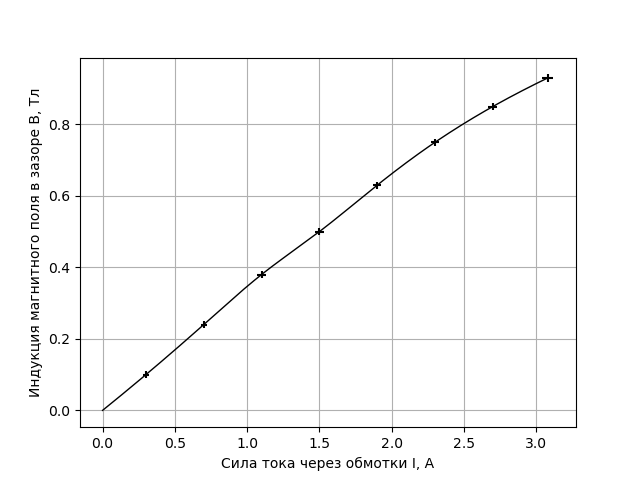
\includegraphics[scale = 0.8]{Curve}
	\caption{Градуировочная кривая $B(I)$ для электромагнита} \label{Кривая}
\end{figure} 

Построим на одном графике зависимости $\left|\Delta P\right|(B^2)$ для меди и алюминия, и на отдельном графике -- такую же зависимость для графита (делаем так из соображений удобства, потому что в случае графита характерные величины перегрузок оказываются на порядок больше). Построенные графики \Ref{Прямые} и \Ref{Графит} приведены ниже.

\begin{figure}[h]
	\centering
	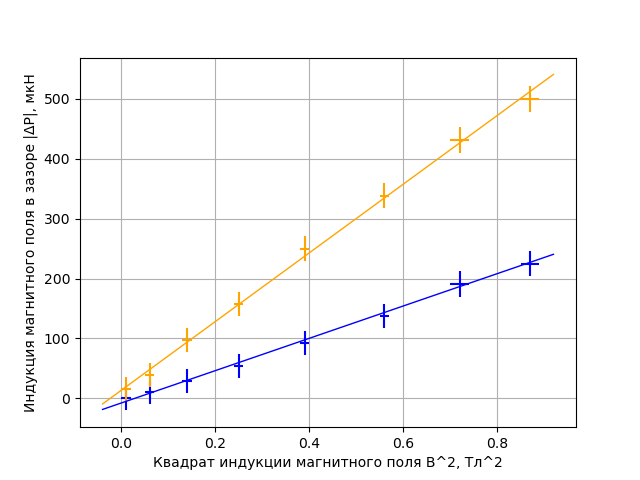
\includegraphics[scale = 0.8]{Plot}
	\caption{График зависимости $\left|\Delta P\right|(B^2)$ для образцов из меди и алюминия (верхняя и нижняя прямые соответственно)} \label{Прямые}
\end{figure} 

\begin{figure}[h]
	\centering
	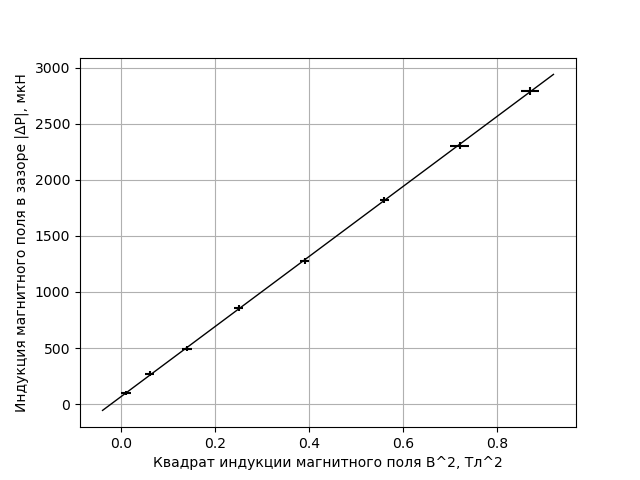
\includegraphics[scale = 0.8]{Plot_Carbon}
	\caption{График зависимости $\left|\Delta P\right|(B^2)$ для образца из графита} \label{Графит}
\end{figure} 

Найдём наклон прямых $\left|\Delta P\right|(B^2)$ и рассчитаем магнитную восприимчивость соответствующих материалов. Погрешности определения этих величин будем находить как $\sigma_k=k\sqrt{\big(\frac{\sigma_{B^2}}{\Delta B^2}\big)^2+\big(\frac{\sigma_{\Delta P}}{\Delta\left(\Delta P\right)}\big)^2}$, где $\Delta B^2$ и $\Delta\left(\Delta P\right)$ -- изменения соответствующих величин в процессе измерений (от минимального до максимального). Так можно сделать, потому что характерные погрешности индукции магнитного поля и перегрузок остаются постоянными. Для меди наклон графика равен $k_{Cu}=\left(2,67\pm0,24\right)\cdot10^{-4}~\frac{1}{\text{Тл}^2}$, отсюда магнитную восприимчивость найдём как $\chi_{Cu}=-\frac{8\mu_0k_{Cu}}{\pi D_{Cu}^2}=-\left(6,5\pm0,8\right)\cdot10^{-6}$ (знак минус совпадает с изначальным знаком перегрузки и соответствует выталкиванию образца из зазора электромагнита). Для алюминия наклон графика равен $k_{Al}=\left(5,73\pm0,26\right)\cdot10^{-4}~\frac{1}{\text{Тл}^2}$, а магнитная восприимчивость -- $\chi_{Al}=\left(2,14\pm0,08\right)\cdot10^{-5}$. Для графита эти же величины равны соответственно $k_C=\left(3,12\pm0,05\right)\cdot10^{-3}~\frac{1}{\text{Тл}^2}$ и $\chi_C=-\left(2,62\pm0,04\right)\cdot10^{-4}$.

Табличные значения магнитной восприимчивости: для меди $\chi_{Cu0}=-6,4\cdot10^{-6}$, для алюминия $\chi_{Al0}=2,2\cdot10^{-5}$, для графита $\chi_{C0}=-2,6\cdot10^{-4}$. Заметим, что все три полученные в эксперименте значения лежат в пределах $1\cdot\sigma$ от табличных, что говорит о корректности и точности измерений.

\section*{Вывод}

В работе были проведены измерения магнитной восприимчивости материалов трёх образцов, сделанных из меди, алюминия и графита. Измерения были проведены по методу Гюи, также была проведена калибровка электромагнита при помощи милливеберметра (получена линейная зависимость в широких пределах). Для магнитной восприимчивости получены значения $\chi_{Cu}=-\left(6,5\pm0,8\right)\cdot10^{-6}$, $\chi_{Al}=\left(2,14\pm0,08\right)\cdot10^{-5}$ и $\chi_C=-\left(2,62\pm0,04\right)\cdot10^{-4}$, из чего можно сделать вывод, что медь и графит являются диа-, а медь -- парамагнетиками. Полученные значения лежат в пределах одного стандартного отклонения от табличных, что говорит о хорошем качестве используемых приборов и проведённых измерений. Стоит отметить, что основным источником погрешности являются инструментальная погрешность электронных весов, однако уменьшить её вряд ли получится, потому что измеряемые величины чрезвычайно малы (порядка $\sim10^{(-5)}~\text{кг}$), к тому же, имеющейся точности вполне достаточно для получения достоверных данных.

\end{document}
